%!TEX root = ./main.tex
\documentclass[11pt, oneside]{book}

\usepackage[utf8]{inputenc}
\usepackage[english]{babel}

% page layout
\usepackage{float}
\usepackage{ragged2e}
\usepackage{rotating}

% toc renaming
\addto\captionsenglish{
  \renewcommand{\listfigurename}{List of figures}
  \renewcommand{\listtablename}{List of tables}
}

% bib
\usepackage[
  backend=bibtex,
  style=ieee,
  maxcitenames=4]{biblatex}
\usepackage{csquotes}
\usepackage[nottoc]{tocbibind}

\addbibresource{references.bib}

% acro, table, lists etc
\usepackage{acronym}
\usepackage{enumitem}
\usepackage{graphicx}
\usepackage{tabularx}
\usepackage{longtable}
\usepackage{array}
\usepackage{multirow}

\usepackage{lscape}

% formatting
\usepackage{color}


% symbols
\usepackage{eurosym}

% refs
\usepackage{hyperref}
\usepackage{cleveref}

% indent
\usepackage{indentfirst}
\setlength\parindent{24pt}

\hypersetup{
  colorlinks=false, pdfborder={0 0 0},
}

\crefname{lstlisting}{listing}{listings}
\Crefname{lstlisting}{Listing}{Listings}

% listings
\usepackage{listings}

% todo
\usepackage{todonotes}

\lstset{frame=tb,
  language=Java,
  aboveskip=3mm,
  belowskip=3mm,
  showstringspaces=false,
  columns=flexible,
  basicstyle={\small\ttfamily},
  numbers=none,
  numberstyle=\tiny\color{gray},
  keywordstyle=\color{blue},
  commentstyle=\color{dkgreen},
  stringstyle=\color{mauve},
  breaklines=true,
  breakatwhitespace=true,
  tabsize=3
}

\begin{document}

%!TEX root = ./main.tex
\begin{titlepage}
	
    \centering
    
\includegraphics[scale = 0.115]{Pictures/logo.jpg}\\[1.7 cm]	% University Logo
    {\Huge Advanced Software Architecture \par}
    \vspace{1cm}
    {\Large Train ticketing system}

    \vfill
    \justifying
    {\large \begin{itemize}[label={}]
        \item Aida Baxhaku (3242528)
        \item Petar Hariskov (3226735)
        \item Alexandra Matreata (3179265)
        \item Eric Rwemigabo (3040356)
    \end{itemize}}
    
    \vspace{2cm}
    \centering
    {\Large \today \par}
    \vspace{0.1cm}
    {\large version 1.0.0}
\end{titlepage}

\frontmatter

\chapter{Revision history}
\label{chp:rev_his}
%!TEX root = main.tex


%!TEX root = main.tex

\tableofcontents

\listoffigures

\listoftables

\chapter{Glossary}
\label{chp:glos}
%!TEX root = main.tex

\begin{acronym}[]
    \acro{ET}{Easy Ticketing}
    

\end{acronym}

\mainmatter

\chapter{Introduction and goals}
\label{chp:intro}
\section{Introduction}
Traveling by train is one of the most common means of transport in the Netherlands and the Western Europe. The majority of people use trains on a daily basis, to go to school, work, etc. It is quite easy and comfortable, but one common problem, that everyone may relate to is the discomfort of train tickets. The printed tickets might get lost, or a passenger might forget to check in, another one is too late to buy one, etc. 

However, we have come up with an alternative train ticket, which will facilitate the journey of many passengers: \ac{ET}. This is a new, promising and innovative technology that suits practically everyone who owns a smartphone. The idea  behind \ac{ET} is very simple: you download an app in your smartphone, open your personal account and connect it to your favorite payment method, and \ac{ET} will do everything else automatically. 

This means, every train will have beacons, which will connect to the passenger’s phones via  bluetooth, it will check the passenger in,  it will automatically calculate the ticket fee and it will reconnect  when the passenger leaves the train. There will be a beacon per every gateway. The beacon can detect the mobile in a diameter of 20m.

The aim of this new technology is to facilitate the journey of train passangers, and take the ticket purchasing to the next level. We plan to implement \ac{ET} firsly in Groningen and after the initial success the aim of our company is to cover the whole Netherlands. 

In this document we are presenting the architecture of our system. In the next chapters you will be introduced to the Stakeholders of the systems and their concerns, the requirements, functional and non-functional.  In section 3, we will briefly analyze the business context and the benefits that \ac{ET} will brings in terms of business. In section 4, the solution strategy is presented, in terms of our main key drivers. Section 5 outlines the building block view, whereas chapter 6 and 7 introduce the runtime and deployment view. The architecture of our system will be concluded with the design decisions and quality scenarios. 

\section{Quality goals}

The top three goals of the architecture of Easy Ticketing whose fulfillment is of highest importance to the major stakeholders (as agreed between them) are listed below:

\textbf{Security} In our system, we could view the importance of security in two major aspects: Firstly, hackers might hack the system and steal money from the account of the train company and secondly, passengers might find a way to fake their tickets. In both cases, this is unacceptable for our customer under any circumstance. Therefore the system must be designed in such way that potential data leaks, which are in theory inevitable, will not result in access to the main database or create damage to the company.

\textbf{Reliability}  Customers are expected to rely on the functioning of Easy Ticketing. Problems with availability of the service are almost as undesirable as security issues, therefore availability must be taken into account throughout the whole system architecture. Breakdown of the system could lead to financial loss for the company, which is in any case not acceptable.

\textbf{Compatibility} Is an important driver for our system. Passengers may be in possession to different smartphones, which may result in incompatibility with the beacon, incompatible frequencies of bluetooth. It is very important to provide the passengers the possibility to purchase the ticket, for as many phone versions as possible.


\chapter{Architecture constraints}
\label{chp:arch_constr}
\input{arch_constraints.tex}

\chapter{System scope and context}
\label{chp:syst_context}
This section outlines the main relations between the system and its environment, external systems or entities with which it interacts. The business and technical contexts in which the system will perform as well as different inter-component communication solutions will be presented in this chapter.

\section{Business context}
\label{sec:business_context}
The system focuses on simplifying the management of information related to train traveling and ticket payment for its users. The system will provide an account for each user which will store information regarding travel distance, destinations, payments, etc. This will help both users travelling by train and the companies providing the travelling services by keeping track of all these components in a centralized manner. 

The system will present the user with the choice of making an automated payment for each trip through the connection between the mobile app and the beacon in the train cart. Alternatively, an external payment system will be presented to the user I every train station where they can log in and perform the transaction. 

A second important target for our system will be represented by companies providing travelling services by train, which may include governmental institutions or different private companies.

\section{Business drivers}
This chapter describes the business forces acting on the system: most important revenue streams and costs and give a justification for the system.

\subsection{Revenue streams}
The main revenue stream for the system will consist of the travel service providers. In order to use the Easy Tickting system, they will have to pay a monthly fee which will include storage and maintenance costs. 

Depending on how well the system usage evolves over time, once enough travel service providers decide to use the system, a small monthly fee can be charged to the user as well. Also, the mobile app functionalities can be improved over time and be accessed by the user over a pay-by-use scenario(e.g. check distances travelled over the last period of time, check fees, see a list of possible price reductions for similar journeys).

\subsection{Costs} 
The costs for the system will be divided in two main groups:
\begin{itemize}
	\item \textbf{development costs:} \\
	these costs will be comprised of installation costs(hardware equipment such as beacons and local servers will be installed and configured inside the trains, central server configuration, backup servers configuration) and software development costs(for the mobile application, databases, computational algorithm for fee calculations).
	\item \textbf{maintenance costs:} \\
	maintenance operations will include constant monitoring of the hardrware equipment(remote monitoring and repairs for components inside the trains and a local team for the central server) and a team for additional functionalities(for the mobile app, optimisations of the computational algorithm, etc).
\end{itemize}



\section{Domain model}
\label{sec:domain_model}
Figure \ref{fig:domain_model} outlines the most significant entities taking part in or being used by the Easy Ticketing system. The system components and their interactions are presented alongside the main external entities needed for different functionalities of the system. The figure also introduces the main actors responsible for the use cases presented in chapter \ref{chp:usecases}.

\begin{figure}[H]
	\centering
	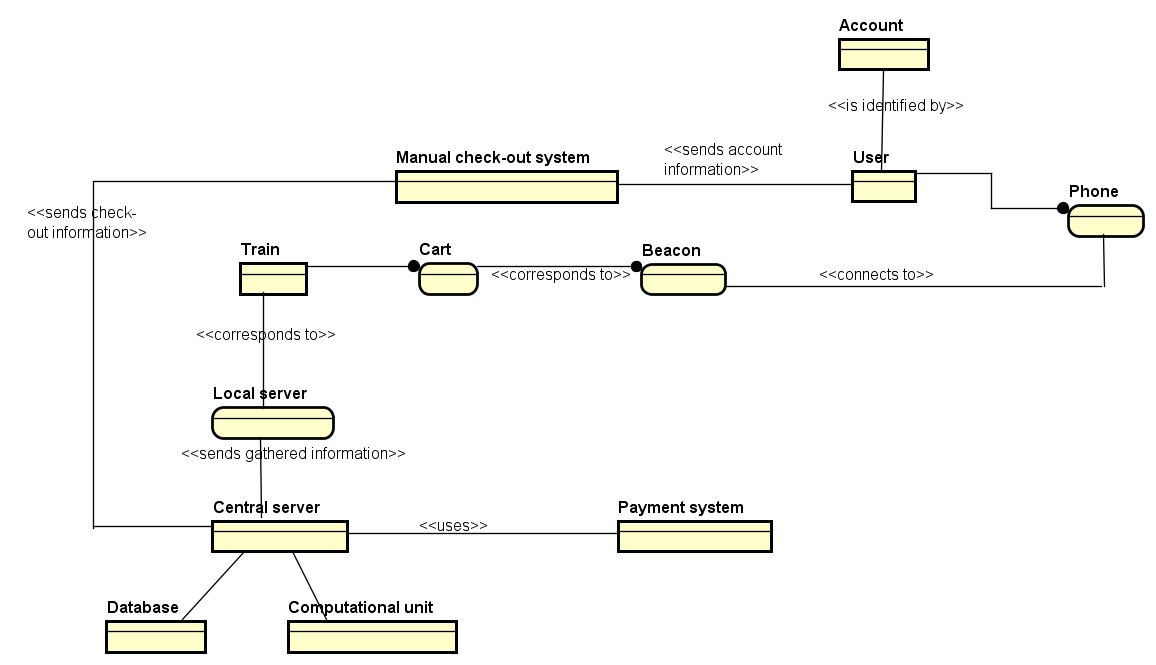
\includegraphics[width=\textwidth]{Pictures/domain_model.png}
	\caption{Domain model}
	\label{fig:domain_model}
\end{figure}

\section{Technical context}
\label{sec:technical_context}
The system will need to perform in a specifically designed technical context consisting of three main environments: a central server collecting all information and performing necessary computations, the setup inside the trains themselves (comprised of beacons and small servers which will collect information per train and send it to the central one every time the train leaves the station) and a login system in each station allowing users to manually check-out of their trip and perform payment.

A set of measures will need to be taken into consideration for the system to be able to operate inside this context by using these different components and environments. These measures will be related to the key attributes required of the system as follows:
\begin{itemize}

\item \textbf{security}: since the system will have access to sensitive information (such as location, financial transactions), every connection between components of the system will need to be secured and trusted. The main connections which will need to be verified each time they are created will be: beacon to mobile application, beacon to server inside the train, small local server to central server. 

\item \textbf{reliability}: for the system to be considered reliable, the main components should be provided with a back-up in case of failure, such as the central server, the beacons in each cart, etc. Also, users should be presented with alternative scenarios in case the main desired activity flow gets interrupted (e.g. possibility to manually check-out of a trip using login system in train station in case of beacon to phone communication being severed)

\item \textbf{compatibility}: the system will need to be compatible with at least the main and most commonly used mobile OS and frequencies 

\end{itemize}

\section{External interfaces}
\label{sec:ext_interfaces}
%!TEX root = main.tex

\begin{table}[H]
  \centering
  \begin{tabularx}{\linewidth}{l|X}
    \textbf{Channel}      & Beacon $\Rightarrow$ Mobile app \\ \hline
    \textbf{Description}  & Beacons detect mobile phones in their proximity having installed the application and initialise a connection.\\ \hline
    \textbf{Connection}   & Bluetooth \\ \hline
    \textbf{Protocol}     & iBeacon \\ \hline
    \textbf{Frequency}    & The train has left a station and a mobile phone is in range of the beacon. \\ \hline
  \end{tabularx}
  \caption{Interface - Beacon to phone}
  \label{tbl:beacon_to_phone}
\end{table}

\begin{table}[H]
	\centering
	\begin{tabularx}{\linewidth}{l|X}
		\textbf{Channel}      & Beacon $\Rightarrow$ Local train server \\ \hline
		\textbf{Description}  & Beacons send information gathered every time a train departs from a station.\\ \hline
		\textbf{Connection}   & Bluetooth \\ \hline
		\textbf{Protocol}     & iBeacon \\ \hline
		\textbf{Frequency}    & The train has left a station. \\ \hline
	\end{tabularx}
	\caption{Interface - Beacon to server}
	\label{tbl:beacon_to_server}
\end{table}

\begin{table}[H]
	\centering
	\begin{tabularx}{\linewidth}{l|X}
		\textbf{Channel}      & Local server $\Rightarrow$ Central server \\ \hline
		\textbf{Description}  & The local server situated inside the train sends information gathered periodically to the central server if an internet connection is possible.\\ \hline
		\textbf{Connection}   & Internet \\ \hline
		\textbf{Protocol}     & UDP \\ \hline
		\textbf{Frequency}    & Once every 20 min or when a connection is possible. \\ \hline
	\end{tabularx}
	\caption{Interface - Local server to central server}
	\label{tbl:local_to_central}
\end{table}

\chapter{Solution strategy}
\label{chp:sol_strategy}
%!TEX root = main.tex

This chapter aims to discuss and present a concrete solution space for the problems described in chapter  \ref{chp:syst_context}. The solutions provided will directly follow the main key drivers of the project and focus on the problem space using views limited only to these most important attributes.

\section{Security}
Different security measures will be taken into account so that the information transferred between different components is not visible to external parties and remains consistent throughout the exchange.

In this manner, the security mechanisms will focus mostly on the interface levels:

\begin{itemize}
	\item \textbf{Beacon to phone:} \\
	Beacons taking part in the system will be uniquely identifiable via its id and mac address. When a phone connects to a beacon, the beacon's identity will be checked against a list of valid beacons by the mobile app. 
	
	Only if the beacon is found in the list, the connection is validated and the mobile app sends the account information to the beacon, thus keeping account information secret from external parties. 
	\item \textbf{Beacon to local server:} \\
	Similarly to the beacon verrification performed by the mobile app once a connection between the beacon and the phone is established, another verification will be performed at the level of the local server.
	
	The local server will check the identity of each beacon sending it information against a list similar to the one available to the mobile app. 
	
	As a second security mechanism, before sending information to the server, the beacons will also check the identity of above mentioned server based on a hashCode. 
	
	\item \textbf{Local to central server:} \\
	Every time the main server receives information from a local server, the identity of the local server will be checked using the hashCode mentioned for the previous connection. 
	
	Also, before sending any information to the central server, every local server will ask the central server to identify itself using a cryptographic key.
\end{itemize}


\section{Compatibility}
The compatibility of the system mainly refers to mobile phones compatibility. The system will take into consideration different types of OS and different frequencies. While not all of these possibilities are taken into consideration, the system will focuss on the most used ones:

\begin{itemize}
	\item OS compatibility(Compatibility-NF-1.1):
	\begin{itemize}
		\item Android
		\item iOS
		\item Windows
	\end{itemize}
	\item frequency: the beacons will send out 10 packages every second(Apple recommendation for optimal retrieval of packages\cite{web:beacons})
\end{itemize}

\section{Reliability}
The reliability of the system takes into consideration 3 main characteristics: availability, fault tolerance and recoverability\cite{iso}.
\begin{itemize}
	\item \textbf{Availability:} \\
	Both the local and central servers will be provided with backup servers. The information stored in the local backup servers will be updated every time the train leaves a station, while the central backup server will be updated more frequently, namely every time the central server receives information from one of the local servers. 
	
	This will allow the backup servers to be fully up to date and to minimize information loss. The backup servers will remain in a passive mode and only become functional once their corresponding main server fails to respond. Once the main server is repaired, information handling will be switched to it and the backup server will return to passive mode.
	
	Every time a main server receives information(local server from beacons and main server from local one), it will notify the senders of having received the packages through a heartbeat signal. If this signal fails to be sent, the backup server will be started.
	
	\item \textbf{Fault tolerance:} \\
	Fault tolerance will be achieved by the system using resource redundancy and duplication of information. By using the backup servers and updating their information regularly, a copy of the information will be stored at all times minimizing information loss. Also, the beacons will be placed in such a manner as to have intersecting range areas, allowing at least two beacons to monitor a specific location in the same time.
	
	\item \textbf{Recoverability:} \\
	By enabling components to keep track of received information packages, the system state is known at each point in time, which allows a very fast detection of defective components. By minimizing error detection time, the recoverability time is also minimized.
\end{itemize}


\chapter{Building block view}
\label{chp:build_block}
%!TEX root = main.tex


\chapter{Runtime view}
\label{chp:runtime}
%!TEX root = main.tex


\chapter{Deployment view}
\label{chp:deployment}
%!TEX root = main.tex


\chapter{Concepts}
\label{chp:concepts}
\section{Domain model}
\label{sec:domain_model}
Figure \ref{fig:domain_model} outlines the most significant entities taking part in or being used by the Easy Ticketing system. The system components and their interactions are presented alongside the main external entities needed for different functionalities of the system. The figure also introduces the main actors responsible for the use cases presented in chapter \ref{chp:usecases}.

\begin{figure}[H]
	\centering
	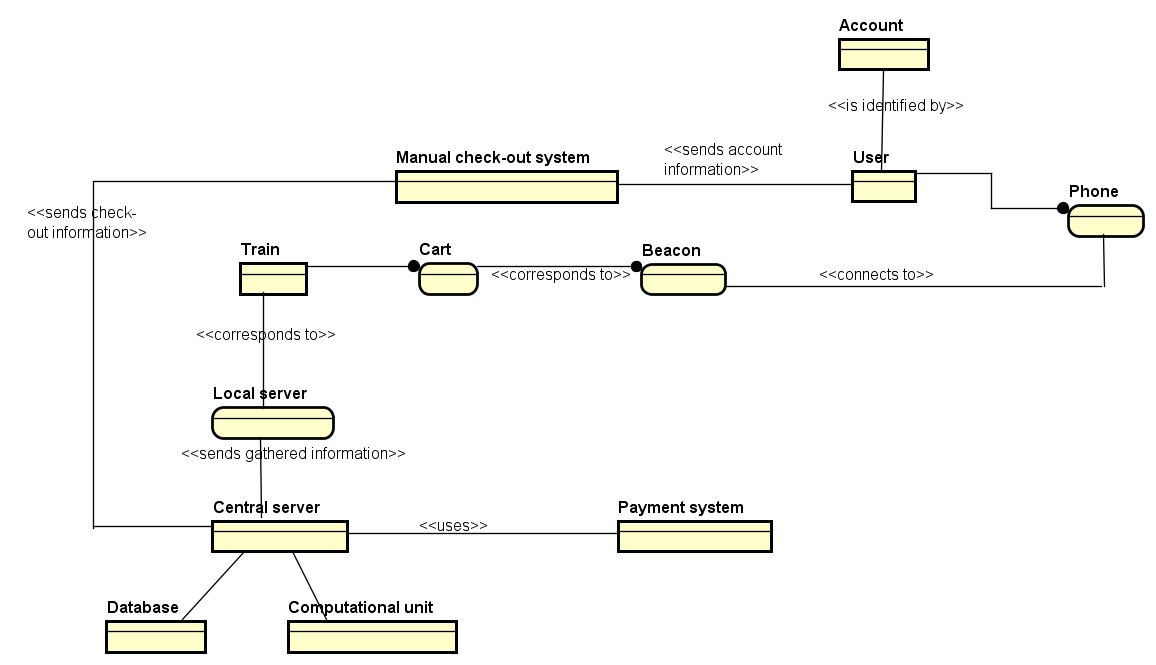
\includegraphics[width=\textwidth]{Pictures/domain_model.png}
	\caption{Domain model}
	\label{fig:domain_model}
\end{figure}

\section{Architectural patterns}
\label{sec:patterns}
%!TEX root = main.tex




\section{Layers}



\label{subchp:layers}


%!TEX root = ../main.tex

\section{Model View Controller}
	The MVC pattern is used to break down the front-end to different pieces each providing different capabilities than the others in order to separate the representation from the logic providing it.


	\subsubsection{Source} \cite{book:design-patterns}


	\subsubsection{Problem}

		Provide an user interface which will allow for different UI capabilities used on different devices with a different purpose. Having mobile devices application which can gives more options to users and stationary units which allow users to log in and out directly at stations.

	\subsubsection{Solution} 

		Break down the UI logic in three separate pieces, namely the model , view and controller, each having one purpose only. The view is responsible with what the user will see, model with connecting to the databases and the business logic and controller with providing controlling logic and managing what view are presented thus allowing for different user interfaces for different devices based on predefined rules in the controller. 


\paragraph{Implications}
\begin{itemize}
	\item decrease performance
	\item increase modularity
	\item increase security
\end{itemize}

\label{sybchp:mvc}

%!TEX root = ../main.tex

\section{Observer Pattern}

\subsubsection{Description of pattern}

	The observer pattern is used to allow an object to publish changes to its state. Other objects subscribe to be immediately notified of any changes to the status of that particular object. 

	
\iffalse
	USAGE : The main server will observe the state of train and Activate the beacons when train leaves a station . We don't need to have the beacons active when at a station 
beacons observe when phones are in range for establishing connections
\fi

\subsubsection{Traceability} 
	% related requirements
	\begin{itemize}
		\item 1
	\end{itemize}

\subsubsection{Source} \cite{book:design-patterns}

\subsubsection{Issue} \label{observerP:issue}
	The most scalable way and also a fault-proof process for management of passengers both for current and ones who have left the train is to have the phone detection work only before and after the train has passed through a station. Having the train server to monitor beacons would make the solution highly unscalable. An operator would have to manually modify the beacons state in the train server himself. On the other hand the beacons should only have to detect nearby phones' bluetooth once or twice a transition between stations making it highly inefficient for them to be active all the time. Having the server monitor and activate all beacons and receive information about passengers would impact the performance of the solution. 

\iffalse

	Therefore there is a clash of requirements which can be solved by implementing a version of a design pattern called the Observer Pattern configured to suit the needs to both be energy efficient and fault-proof. 

	This however creates an issue that the beacons should be allowed to operate on their own and they should also monitor the state of the train.
 \fi


\subsubsection{Solution} 
	The solution to the problem listed in the \ref{observerP:issue} paragraph would be to server monitor the train and the beacons to listen to events passed through the server. The server will allow the beacons to observe its state and listen to changes in the behaviour. This could be implemented via a design pattern called Observer Pattern explained in more detail in paragraph \ref{observerP:rationale}


\subsubsection{Rationale} \label{observerP:rationale}
	Even though the Observer Design Pattern is a pattern related to coding and resolves coding issues this section look at the pattern from a different perspective. The architecture of the solution described in this document uses the Observer Pattern to allow the beacons in the train to monitor the state of the train itself. Once the train has left the station the train server will change the status to 'departed' and through attached listeners, the beacons will start their main functionality - to echo for discovered bluetooths in the particular cart they are located in.

\subsubsection{Implications}
\begin{itemize}
  \item 
\end{itemize}


\label{subchp:observerP}


\section{Replicated system}
\label{subchp:replicatedP}

%!TEX root = ../main.tex


\section{Trusted subsystem}

Trusted Subsystem : The phone needs the credentials of the beacon in order to send its credentials back to it . The beacon receives credentials from the phone and registers it in the system. 
	
\label{subchp:trustedP}


\section{Security}
\label{csec:security}
%!TEX root = main.tex


\section{Compatibility}
\label{sec:compatibility}
%!TEX root = main.tex


\section{Reliability}
\label{sec:reliability}
%!TEX root = main.tex


\chapter{Design decisions}
\label{chp:design_decisions}
%!TEX root = main.tex


\chapter{Quality scenarios}
\label{chp:quality_scenarios}
%!TEX root = main.tex


\listoftodos[Notes]

\appendix

\chapter{Time tracking}
\label{chp:time_track}
%!TEX root = main.tex

\begin{table}[H]
	\centering
	\begin{tabularx}{\textwidth}{p{2cm}|X|p{2.5cm}}
		\textbf{Member} & \textbf{Task} & \textbf{Time (hrs)} \\
		\hline
		ab &Introduction and goals                  & 8 \\
		   &Requirements, Key Drivers, Stakeholders & 9  \\
		   &Baseline Architecture: Security Tactics & 7  \\
		   &Software Architecture: Logical view     &12   \\
		   &Evaluation: Utility tree, scenarios     & 9  \\

		& & \textbf{45} \\
		\hline
		ph &  &  \\
			& Architectural Patterns & 22 \\
		& & \textbf{22} \\
		\hline
		am & system scope and context & 10 \\
		 & functional requirements & 3 \\
		 & solution strategy & 6 \\
		 & reliability tactics & 3 \\
		 & process view & 6 \\
		 & use cases & 7 \\
		& & \textbf{35} \\
		\hline
		er & Evaluation, Design decisions, compatibilitytactics & 21 \\
		& & \textbf{21} \\
		\hline
	\end{tabularx}
	\caption{Time tracking}
	\label{tab:timetracking-1}
\end{table}


\backmatter

\printbibliography

\end{document}
